\scanpage{60}
\S 1 Ch. de De Rham ordinaire

\S 2 Tour d'horizon sur Ch. $\ell$-adiques. Motivations pour le désir d'une coh. $p$-adique en car. $p$.

\S 3 \unsure{Tapis} de Washnitzer-Monsky.

\S 4 Stratifications. Relations de W.M. avec connexions de Gauss-Manin sur coh. de De Rham

\S 5 \deleted{\unsure{Le}} Site cristallin et site stratifiant. Énoncé \deleted{de} d'un théorème et d'une conjecture en car. nulle.

\S 6 Calculs \v{C}echistes (car. quelconque).

\S 7 Comparaison de la Ch. de De Rham et cristalline (car. \unsure{nulle}).

\S 8 \deleted{Comparaison} \inserted{Retour} sur le cas de la car. $p>0$

\figure{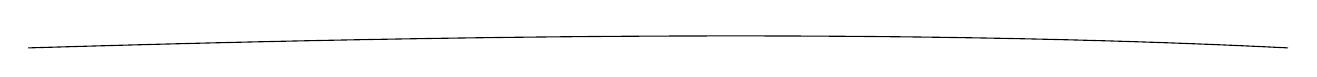
\begin{tikzpicture}
\draw (0,0) .. controls (5,.15) and (11,.25) .. (16,0);
\end{tikzpicture}}

\margin{\deleted{\uline{\unsure{Ch. strat.}}}\\
\uline{Ch. stratifiante}}

6.1. Commençons à travailler sur le topos \uline{stratifiant} pour $X/S$. Il y a l'objet $\widetilde X$ de ce topos: il \uline{couvre l'objet final} (c'est ici qu'on utilise la restriction sur les objets du site stratifiant par rapport à ceux du site cristallin). Donc suite spectrale de Leray
\[
H^*(X_{\mathrm{strat}},F)\Longleftarrow E_2^{pq}
=H^p(\nu\mapsto H^q(\widetilde X^{\nu+1},F)).
\]
Or on constate que
\figure{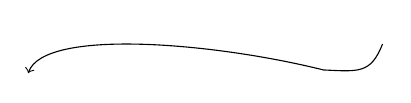
\begin{tikzpicture}
\draw[->] (4.5,.25)..controls (4.35,-.13) and (4.2,-.1)..(3.75,-.08)..controls (2.35,.27) and (.2,.45)..(0,-.12);
\end{tikzpicture}}
\[
\widetilde X^{\unsure{\nu}+1}
=\varinjlim_i\deleted{\unsure{\widetilde X}}\,
\underbrace{\Delta_X^{(\unsure{\nu})}(i)}_{
\substack{\text{voisinage inf. ième}\\
\text{de la diagonale dans}\\
X^{\nu+1}}}
\,\deleted{\unsure{X}}.
\]
\inserted{considéré comme \unsure{pro-objet} de $X$}
\deleted{$\unsure{X\longrightarrow}$}
\diagram{\begin{tikzcd}[ampersand replacement=\&,column sep=small,row sep=small]
X \& U\arrow[l]\arrow[dr] \&\\
\&\&X'
\end{tikzcd}}

D'autre part, pour tt objet $(U,X')$ du site stratifiant, on \unsure{aura}

\margin{59}
